\section{Główny skrypt}

Skrypt główny jest zasadniczo podzielony na kilka części. Jego szczegółowy algorytm działania przedstawiony
jest na rysunku 1. Po pierwsze, uruchamia on model podziału sieci pomiędzy dzierżawców.
W wyniku tego otrzymujemy podgrafy dla każdego z klientów, które są następnie przekazywane
do modelu alokacji przepływów jako stała wejściowa. W przypadku znalezienia rozwiązania,
dla danej podzielonej sieci sprawdzane są parametry jakości obsługi takie jak opóźnienie
oraz jitter. W przypadku nie spełnienia tych wymagań, algorytm bierze następne najlepsze rozwiązanie z drugiego modelu i dla niego zostają sprawdzone
parametry QoS. Jeśli dla żadnego rozwiązania z puli nie otrzymamy zadowalających rezultatów,
algorytm powraca do pierwszego modelu i wybiera z jego puli rozwiązań kolejną najbardziej
optymalnie podzieloną sieć, a następnie przekazuje te dane do modelu drugiego.
Cykl ten powtarzany jest do znalezienia pasującego rozwiązania.

\begin{figure}
\centering
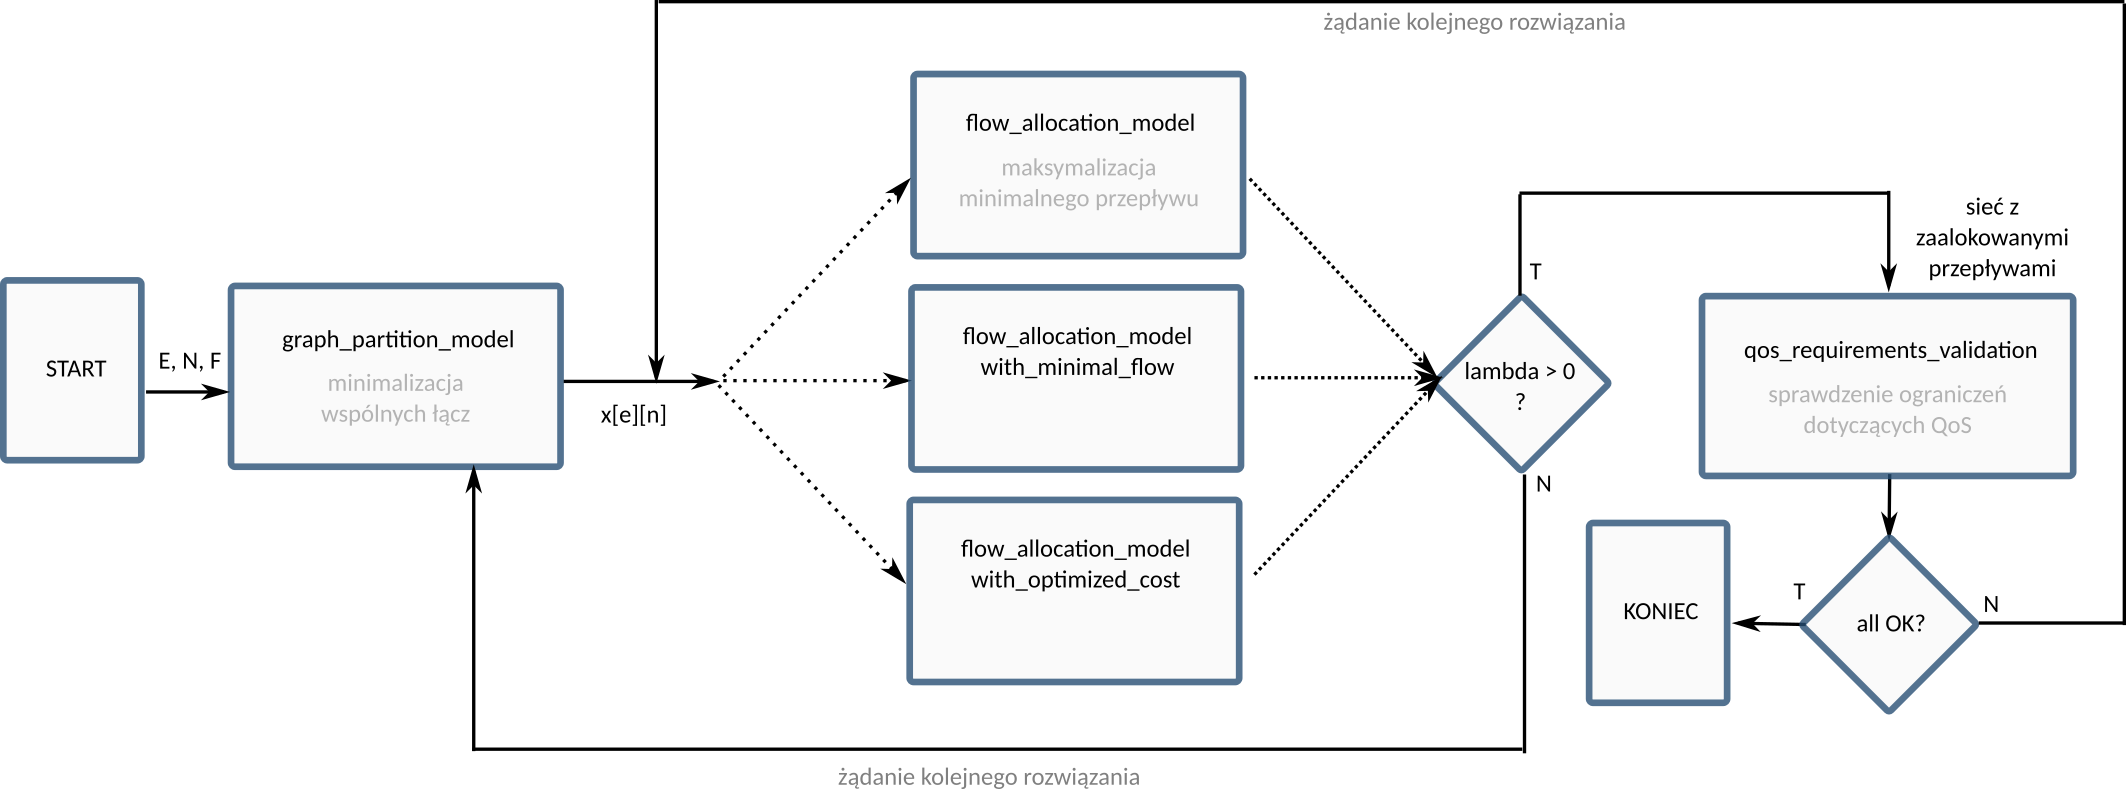
\includegraphics{scheme_rendered.png}
\end{figure}

Dodatkowo z powodu ograniczeń języka OPL musieliśmy zaimplementować własne funkcje
takie jak obliczanie wariancji czy sortowanie.
